\chapter*{Results}
\addcontentsline{toc}{chapter}{Results}\label{cap:res}

\section*{Preliminary TCR repertoire analysis}
\addcontentsline{toc}{section}{Preliminary TCR repertoire analysis}


\begin{figure}[!t]
	\centering
	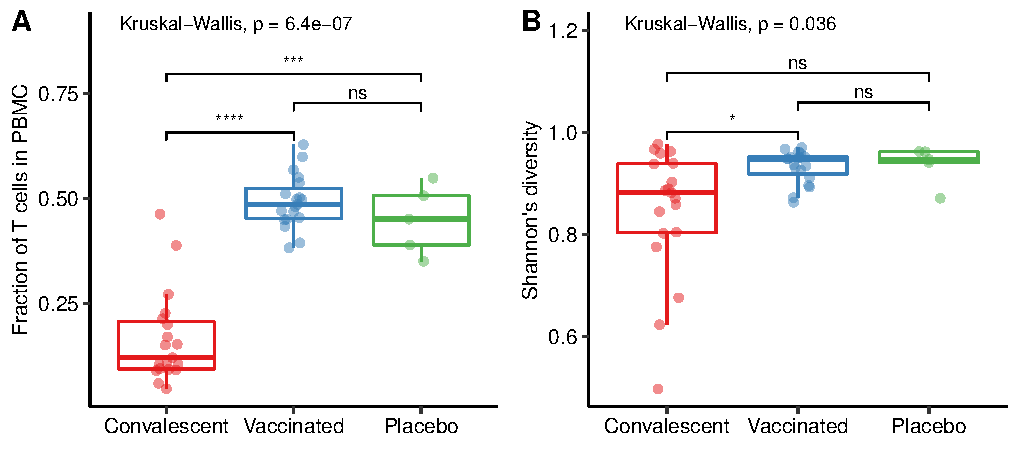
\includegraphics[width=0.7\textwidth,keepaspectratio]{figures/fig1.pdf}
	\caption{\textbf{TCR repertoire preliminary analysis. (a)} Fraction of T cells among peripheral blood mononuclear cells (PBMC). \textbf{(b)} Simpson clonality index. A value closer to 1 indicates the emergence of a few dominant clones, whereas it reaches its minimum when TCR frequencies are evenly distributed. Statistical significance was determined by two-sided Wilcoxon rank-sum tests. N = 43 independent samples (19 SARS-CoV-2 convalescent individuals, 19 Ad26.COV2.S vaccine recipients, 5 placebo recipients).}
	\label{fig:lymphopenia}
\end{figure}
%%% Pvalues asterisk equivalence?

% One of the clinical characteristics of \covid-infected patients is lymphopenia or low lymphocyte counts in peripheral blood, specially affecting to T cells. The degree of lymphopenia correlates with disease severity, and it is usually associated with a pro-inflamatory cytokine storm \citep{lymphopeniaseverity}. It is hypothesized that the underlying causes of lymphopenia can be the pro-inflamatory cytokine levels, exhaustion of T cells upon COVID-19 infection and direct \covid-infection of T cells \citep{lymphopenia}.

One of the clinical characteristics of \covid-infected patients, lymphopenia, can be observed from a TCR repertoire analysis perspective. In TCR repertoire sequencing from a peripheral blood sample, both the number of nucleated cells and total T cells can be estimated by the amplification of reference gene primers. The fraction of T cells was significantly lower in convalescent individuals compared to vaccinated and placebo ($p = 2.5\cdot10^{-9}$ and $p = 5.6\cdot10^{-4}$, two-sided Wilcoxon rank-sum test) and no significant differences were observed between vaccinated and placebo subjects (Fig. \ref{fig:lymphopenia}a). Some convalescent patients \TCRB{} repertoires had a higher clonality (Fig. \ref{fig:lymphopenia}b), indicating that a few clones were expanded and possibly reflecting that these individuals have had a recent adaptive immunity response, most likely to \covid{} infection.

%%% Sentence about lymphopenia affecting repertoire landscape???





\section*{Breadth and depth of \covid-specific T cell response}
\addcontentsline{toc}{section}{Breadth and depth of \covid-specific T cell response}


\begin{figure}[!t]
	\centering
	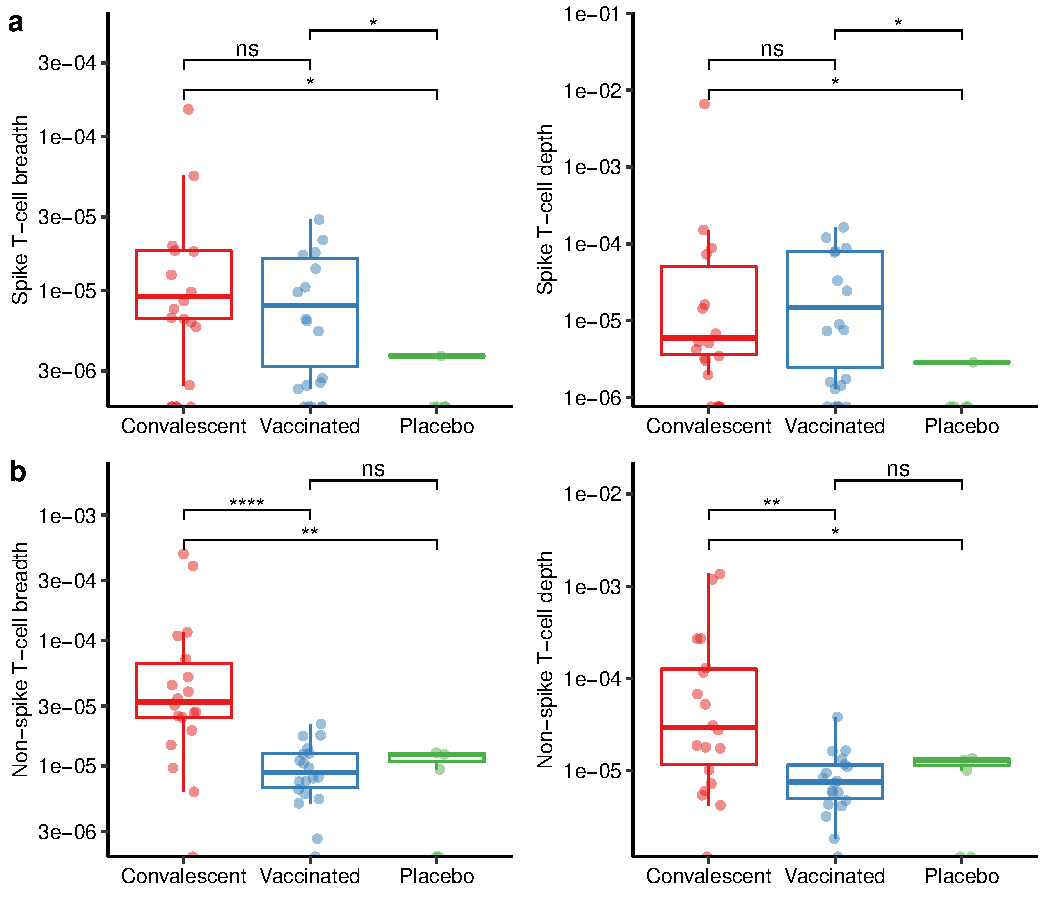
\includegraphics[width=0.7\textwidth,keepaspectratio]{figures/fig2.pdf}
	\caption{\textbf{\covid-specific \TCRB{} repertoire analysis. (a)} Spike-specific T cell breadth and depth. \textbf{(b)} Non-spike-specific T cell breadth and depth. Breadth was calculated as the fraction of unique TCR sequences specific to spike / non-spike proteins; depth is the relative frequency of those specific TCRs in the repertoire. Statistical significance was determined by two-sided Wilcoxon rank-sum tests. N = 43 independent samples (19 SARS-CoV-2 convalescent individuals, 19 Ad26.COV2.S vaccine recipients, 5 placebo recipients)}
	\label{fig:bd}
\end{figure}

To evaluate the magnitude of the T cell response to \covid{} after disease and vaccination, TCR repertoires of convalescent, vaccinated and placebo recipients individuals were annotated with CD8\textsuperscript{+} and CD4\textsuperscript{+} TCR datasets that had previously been determined to be \covid-specific and screened for enrichment compared to a background of healthy individuals repertoires in order to remove TCRs that may be unspecific (i.e. cross-reactive to common antigens) (See \nameref{cap:met}). Among the 43 repertoires analyzed there were 11,604,850 distinct TCR sequences (V gene + CDR3 aminoacid sequence) of which only 284 were \covid-specific. Out of these annotated 284 TCRs, 51 were public (i.e. present in more than one individual).

Responses to \covid{} spike and non-spike were measured in terms of breadth (unique TCR sequences) and depth (frequency of those TCRs). Both convalescent and vaccinated subjects had a higher and undistinguishable spike-specific response compared to placebos in terms of breadth and depth (Fig. \ref{fig:bd}a). By contrast, breadth and depth of non-spike TCRs were significantly higher in convalescent individuals versus vaccinated and placebos, and there were no significant differences between the latter two (Fig. \ref{fig:bd}b), as expected because Ad26.COV2.S vaccine only carry the spike antigen.


\begin{figure}[!t]
	\centering
	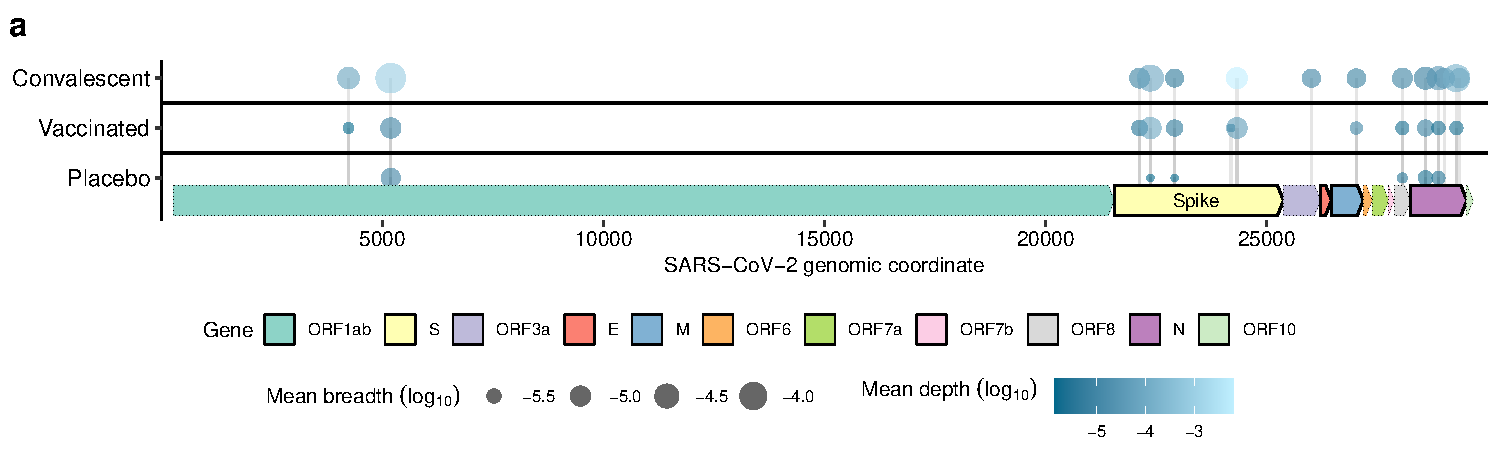
\includegraphics[width=\textwidth,keepaspectratio]{figures/hits.pdf}
	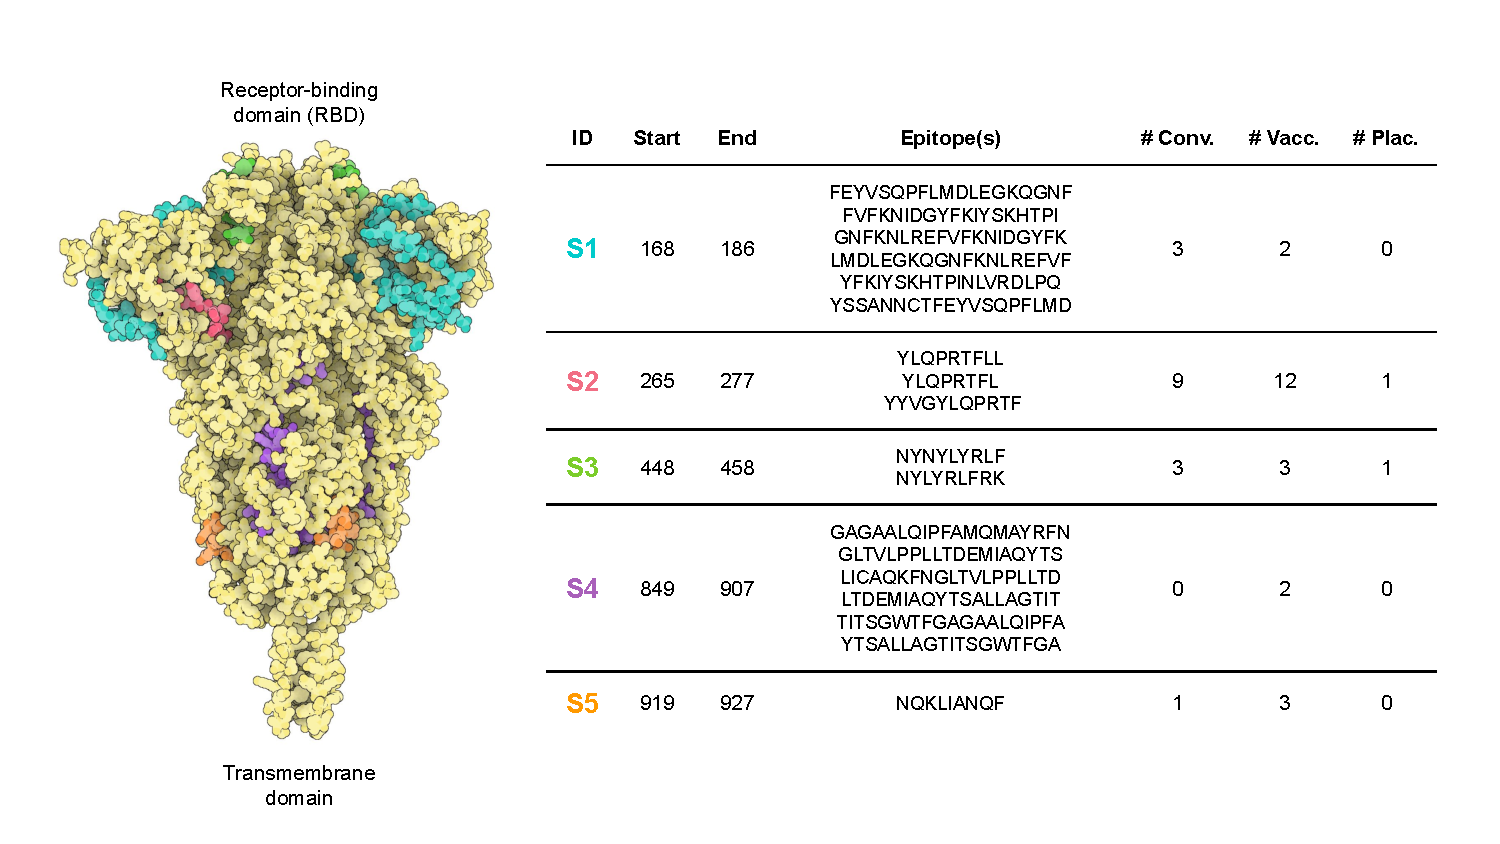
\includegraphics[width=0.7\textwidth,keepaspectratio]{figures/spike_w_table.pdf}
	\caption{\textbf{Epitopes recognized by T cells accross SARS-CoV-2 genome. (a)} Lollipop plot of the \TCRB{} \covid{} specificity in convalescent, vaccinated and placebo individuals accross the coronavirus genome. Size of the dots indicate the mean breadth accross all samples in a group and color scale indicates the mean depth of the response. Genes outlined with solid lines are structural (S, E, M and N), whereas dotted ones encode non-structural proteins. \textbf{(b)} Localization and characteristics of the 5 \covid{} spike epitopes recognized by TCRs in this study. Epitopes appear colored in the three monomers of a spike protein 3D representation (PDB: 6XR8, side view). Start, End: epitope protein coordinates (1-based); \# Conv., \# Vacc., \# Plac.: number of individuals in a group with TCRs specific to that epitope.}
	\label{fig:hits}
\end{figure}

An in-depth analysis of the genomic localization of \covid{} epitopes recognized by TCRs revealed that most of the T cell immune response in convalescent individuals was directed towards structural proteins S and N (Fig. \ref{fig:hits}a). Although vaccinated subjects showed some response to non-spike proteins, for most epitopes this signal was less broad and deep compared to the convalescent group and most likely due to unspecific annotations or cross-reactivity, since placebo recipients also showed a minimal level of response. The localization of the 5 spike protein epitopes is shown in Fig. \ref{fig:hits}b. As opposed to B-cell epitopes, T cell epitopes localization was not restricted to the protein surface since TCRs recognize antigens processed and presented in MHC molecules by human cells, and it was shown in the spike protein 3D representation, where most of the epitopes were partially (S1, S3, S5) or completely (S2, S4) buried in the structure. S2 epitope was in fact the most widely recognized by convalescent (9/19) and vaccinated (12/19) individuals, and S4, the most hidden in the protein, was unrecognized by convalescent subjects and exclusively recognized by TCRs of 2 out of 19 vaccine recipients.




\section*{TCR similarity network analysis}
\addcontentsline{toc}{section}{TCR similarity network analysis}


\begin{figure}[!t]
	\centering
	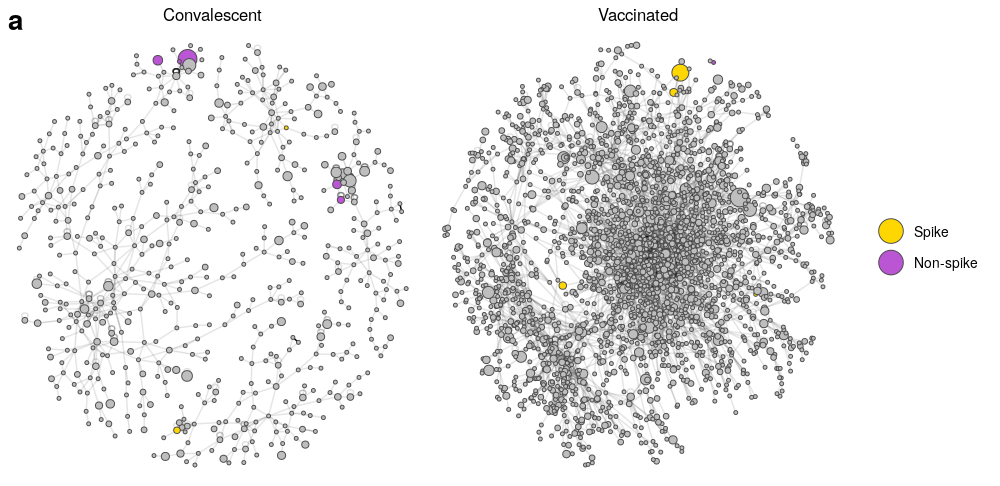
\includegraphics[width=0.8\textwidth,keepaspectratio]{figures/two_nets.png}
	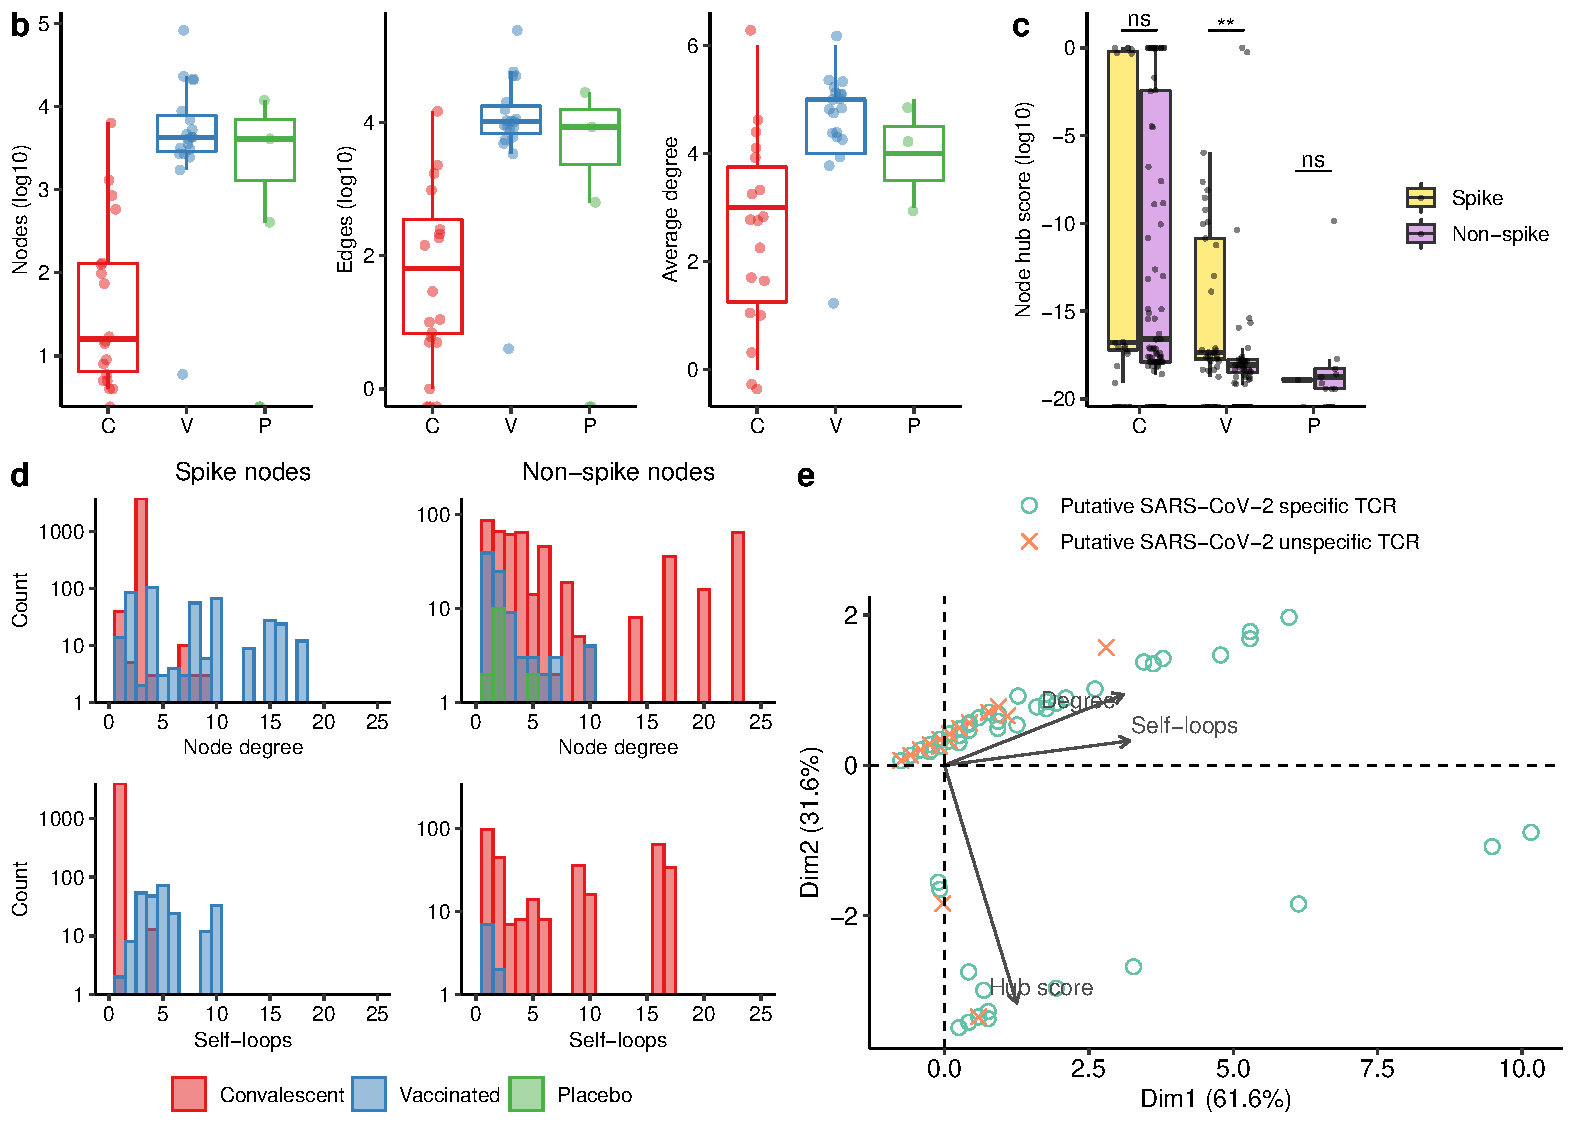
\includegraphics[width=\textwidth,keepaspectratio]{figures/fig4.pdf}
	\caption{\textbf{\covid-specific \TCRB{} similarity networks. (a)} \TCRB{} similarity networks as undirected graphs, where each node represents a unique V gene + CDR3 aminoacid sequence combination. Only \covid-specific nodes (colored) and the nodes in their components (gray) are shown for convalescent subject 18 and vaccinated subject 12. Two nodes are connected by and edge if their tcrdist3 distance is $\leq$ 12. Loops (self-edges that start and end at the same node) represent additional unique nucleotide sequences encoding the same V gene + amino acid sequence (i.e., convergence). Node size represents the TCR frequency. \textbf{(b)} Distribution of network global properties by group. \textbf{(c)} Spike and non-spike nodes hub score distributions by group. \textbf{(d)} Histograms of \covid-specific nodes degree and self-loops. Y axis represent node counts taking their frequency into account. \textbf{(e)} Putative \covid-specific and unnspecific biplot based on network local metrics. A node was putatively considered \covid-specific if it was a spike node in a convalescent or vaccinated network, or if it was a non-spike node in a convalescent network.  C: convalescent, V: vaccinated, P: placebo.}
	\label{fig:nets}
\end{figure}


The landscape of TCR repertoires is vast and complex. A simple antigen specificity annotation by V gene and CDR3 aminoacid sequence exact match, although informative and straightforward, can underestimate the magnitude of the T cell response. In order to capture the \covid-specific TCR repertoire architecture, graphs representing networks of similar TCRs were generated for the 43 TCR repertoires. Fig. \ref{fig:nets}a shows two \covid-specific TCR sequence similarity networks of one convalescent and one vaccinated individual. A \covid-specific TCR similarity network is defined as all the components (subgraphs in which any two nodes are connected to each other by paths) that include at least one \covid-specific node (yellow, purple). Spike-specific nodes are present in both graphs, while non-spike-specific nodes are restricted to the convalescent individual, as expected. In both networks, some \covid-specific nodes had a high relative frequency, represented by node size in the graph. As for the networks architecture, the most striking difference was the network size, with the convalescent graph having less edges and nodes that the vaccinated one. This was also observed at the group level, and furthermore, convalescent \covid-specific TCRs networks had a lower average degree (number of edges per node) compared to vaccine and placebo recipient individuals (Fig. \ref{fig:nets}b).

In this work, it has been noted that direct annotation with \covid-specific TCRs is not very precise, since there was some non-spike response in vaccine recipients, as well as response to some \covid{} epitopes in healthy placebo recipients (Figs. \ref{fig:bd}b, \ref{fig:hits}a). Network analysis can help identifying those nodes that truly are \covid-specific versus those that may be cross-reactive. It was expected for spike-specific TCRs to have more importance in convalescent and vaccinated subjects networks compared to placebo, and for non-spike-specific TCRs to be relevant only in convalescent individuals. Important nodes in network science are known as hubs, or nodes with a number of edges exceeding the average, and the network local property that measures this quality is the hub score, which takes into account how well connected is a node itself, and those nodes that it is connected to. In convalescent and placebo subjects, there were no significant differences in hub scores distributions of spike-specific and non-spike specific nodes, beign the hub scores very low in the placebo recipient \covid-specific nodes. However, hub scores were significantly greater for spike-specific nodes in vaccinated individuals compared to non-spike-specific nodes ($p = 2.1\cdot10^{-3}$, two-sided Wilcoxon rank-sum test) (Fig. \ref{fig:nets}c). This suggests that TCRs annotated as non-spike-specific in vaccine recipient subjects or any \covid-specific TCR in the placebo group do not have an important role in their TCR repertoires and may be \covid-unspecific and cross-reactive.

In addition, the spike-specific nodes with highest degrees (more connections) were from vaccinated subjects, whereas the highly connected non-spike-specific nodes belonged to convalescent individuals (Fig. \ref{fig:nets}d, top panels). The same trend was observed for self-loops, which represent TCR convergence, i.e. additional nucleotide TCR sequences encoding the same V gene + amino acid sequence (Fig. \ref{fig:nets}d, bottom panels). Together, all these network properties facilitate the differentiation between putative \covid-specific TCRs (spike-specific detected in convalescent and vaccinated individuals and non-spike-specific detected in convalescent subjects) and putative \covid-unspecific TCRs (those detected in placebo repertoires and non-spike-specific in vaccine recipients) (Fig \ref{fig:nets}e). Nevertheless, due to the constantly changing nature of the TCR repertoires, after a time period following antigen exposure, some putative \covid-specific TCRs can be undistinguishable from putative unspecific ones in terms of hub score, degree and self-loops, since they become less important in the adaptive immunity landscape once the infection is cleared.



% \textcolor{lightgray}{\lipsum[1-2]}
